\documentclass[11pt]{article}

    \title{%
    \Huge \vspace{60mm}\textbf{Manual del Usuario} \\
    \huge Software de gestión de Cuenta Bancaria}
    \date{}

    \addtolength{\topmargin}{-3cm}
    \addtolength{\textheight}{3cm}
    \usepackage{fancyhdr}
    \usepackage{geometry}
    \geometry{
        a4paper,
        total={170mm,257mm},
        left=20mm,
        top=20mm,
    }
	\usepackage{graphicx}
	\usepackage{caption}
\begin{document}

% Portada
\maketitle
\thispagestyle{empty}
\pagenumbering{gobble}
\newpage
% Sección de funcionalidades software
\section{Funcionalidades}
La presente guía tiene por objetivo orientar al usuario en la correcta utilización del software de gestión de Cuenta Bancaria, el cual se distribuye en un archivo \(.jar\). El mismo software puede ejecutarse tanto en Windows como en Linux o macOS. Su propósito es computar transacciones bancarias a través de su monto y una descripción opcional, y brindar opciones de filtro sobre las mismas, por ejemplo, para mostrar la transacción más antigua o la más costosa. La interfaz de usuario es simple e intuitiva, para evitar distracciones y que su utilización no conlleve mayores inconvenientes.
% Sección de uso del programa (y la GUI)
\section{Uso del programa}
Al ejecutar el archivo \(SoftwareDeGestion.jar\), se le pedirá la respectiva clave de acceso. En caso de ingresarla erróneamente, el programa se bloqueará, con lo cuál deberá cerrarlo y ejecutarlo nuevamente para volver a ingresar la clave. Finalmente, accederá a la pantalla principal del programa. Sus elementos se detallan a continuación.
\begin{figure}[htp]
\centering
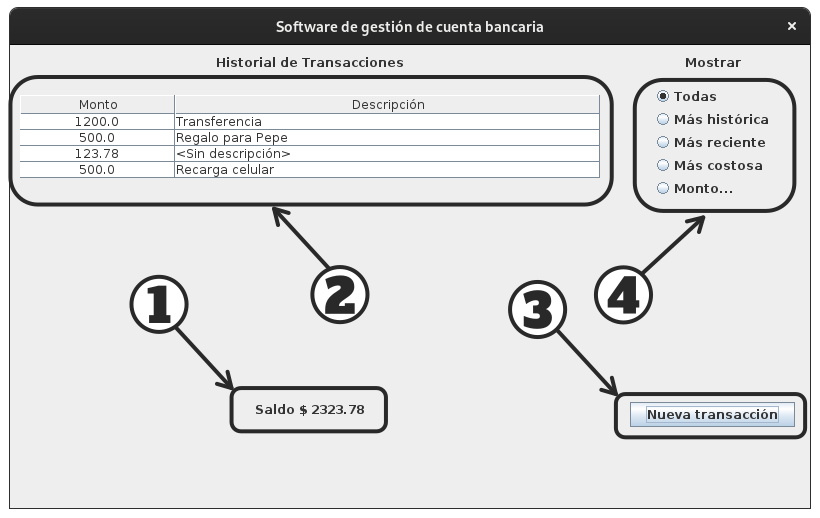
\includegraphics[scale=0.75]{programa.png}
\caption*{\emph{Ventana principal de la aplicación}}
\label{}
\end{figure}
\begin{enumerate}
	\item Saldo actualizado al día de la fecha.
	\item Historial de transacciones con monto y descripción.
	\item Botón para ingresar una nueva transacción. Debe tener en cuenta que los montos deben ser números. El símbolo decimal es el punto. El monto es obligatorio.
	\item Opciones de filtrado del historial de transacciones. Por defecto se observan todas las transacciones efectuadas, pero puede optarse por ver la más histórica, la más reciente, la más costosa, o todas las que tengan un monto determinado. Los filtros son excluyentes entre sí.
\end{enumerate}
\end{document}
